\documentclass[12pt,twoside]{report}
\usepackage[utf8]{inputenc}
\usepackage{graphicx}
\usepackage{acronym}
\usepackage{ae,aecompl}
\usepackage{acronym}
\usepackage[fleqn]{amsmath}
\usepackage{amssymb}
\usepackage[compatibility=false]{caption}
\usepackage[T1]{fontenc}
\usepackage{graphicx}
\usepackage{subcaption}
\usepackage{color}
\usepackage[a4paper,width=150mm,top=30mm,bottom=30mm,bindingoffset=12mm]{geometry}

\usepackage{xcolor}
\usepackage{gensymb}
\usepackage{bm}
\usepackage{etoolbox}
\usepackage[inline]{enumitem}	% To enumerate within a single line
\usepackage{float}

\usepackage{fancyhdr}
\pagestyle{fancy}
\fancyhead[LE,RO]{\itshape \nouppercase \rightmark}
\fancyhead[LO,RE]{\itshape \nouppercase Chapter \arabic{chapter}}

\usepackage{setspace}
\doublespacing

\usepackage{gensymb}
\usepackage{hyperref}
\usepackage{etoolbox}
\usepackage{mathtools}

\usepackage{datetime}

\usepackage[inline]{enumitem}	% To enumerate within a single line
\usepackage{amssymb}  % Extra maths symbols
\usepackage{bm}
\usepackage{hyperref}
\usepackage[square,numbers]{natbib}

\acrodef{DNS}{double neutron star}
\acrodefplural{DNS}[DNSs]{double neutron stars}
\acrodef{HR}{Hertzsprung-Russell}

\def\apj{Astrophys.~J.}
\def\mnras{Mon.~Not.~R.~Astron.~Soc.}
\def\aapr{Astron.~Astrophys.~Rev.}

\newdateformat{monthyeardate}{%
  \monthname[\THEMONTH], \THEYEAR}


\usepackage{arydshln}
\usepackage{filecontents}

\newcommand{\mdash}{-}


\graphicspath{ {Figures/}, {Figures/Introduction/}}

\begin{document}

	\begin{titlepage}
    \begin{center}
        \vspace*{2cm}
        \large
        % \textbf{On the Evolution and Fate of Interacting Massive Binary Stars}
        \textbf{TITLE OF THE THESIS}
		
        \vspace{0.5cm}
        by
        \vspace{0.5cm}

        \large
        \textbf{ALEJANDRO VIGNA-G\'OMEZ \\ \& \\ JAMES WILLIAM BARRETT}
		
        \vspace{5cm}

        A thesis submitted to the University of Birmingham for the degree of DOCTOR OF PHILOSOPHY

        \vfill

        % \includegraphics[width=0.6\textwidth]{crest}

        \vspace{2cm}

        \end{center}

        \begin{flushright}
        % \large
        Institute for Gravitational Wave Astronomy \\
		School of Physics and Astronomy \\
		College of Engineering and Physical Sciences \\
        University of Birmingham \\
        \color{red}{Date}
        \end{flushright}
\end{titlepage}


	\pagenumbering{roman}
	
	\begin{flushleft}
	{\LARGE\textbf{Abstract}\\}
\end{flushleft}

This thesis vastly improved the knowledge of humanity, while revolutionising several fields in the meantime. 
	\begin{flushleft}
	{\LARGE\textbf{Dedication}\\}
\end{flushleft}

To Alejandro Vigna-G\'omez and James William Makepeace Barrett III.
	\begin{flushleft}
	{\LARGE\textbf{Acknowledgements}\\}
\end{flushleft}

\begin{flushright}
``Cheesy quote."
\end{flushright}

Funding for my studies was provided by the University of Birmingham.
	
	\tableofcontents
	\setlength{\parskip}{18pt}
	\addcontentsline{toc}{chapter}{List of Figures}
	\listoffigures
	\addcontentsline{toc}{chapter}{List of Tables}
	\listoftables

	\clearpage

	\pagestyle{fancy}
	\fancyhead[LO,LE]{\nouppercase{\rightmark}}
\pagenumbering{arabic}

\chapter{Introduction}
\label{chap:introduction}
For a circular orbit, we can equate the centripetal force $F_{\rm c,i}= m_ir_i\dot{\theta}^2$ to the gravitational force $F_{\rm g}=Gm_1m_2/r^2$, and solve for $\dot{\theta}^2$ in order to derive Kepler's Third Law in the form
\begin{equation}\label{eq:Chap1:keplerThirdLaw}
	\dot{\theta}^2 = \dfrac{G M}{r^3}.
\end{equation}

Equation \ref{eq:Chap1:keplerThirdLaw} is Kepler's Third Law.

\begin{figure}
	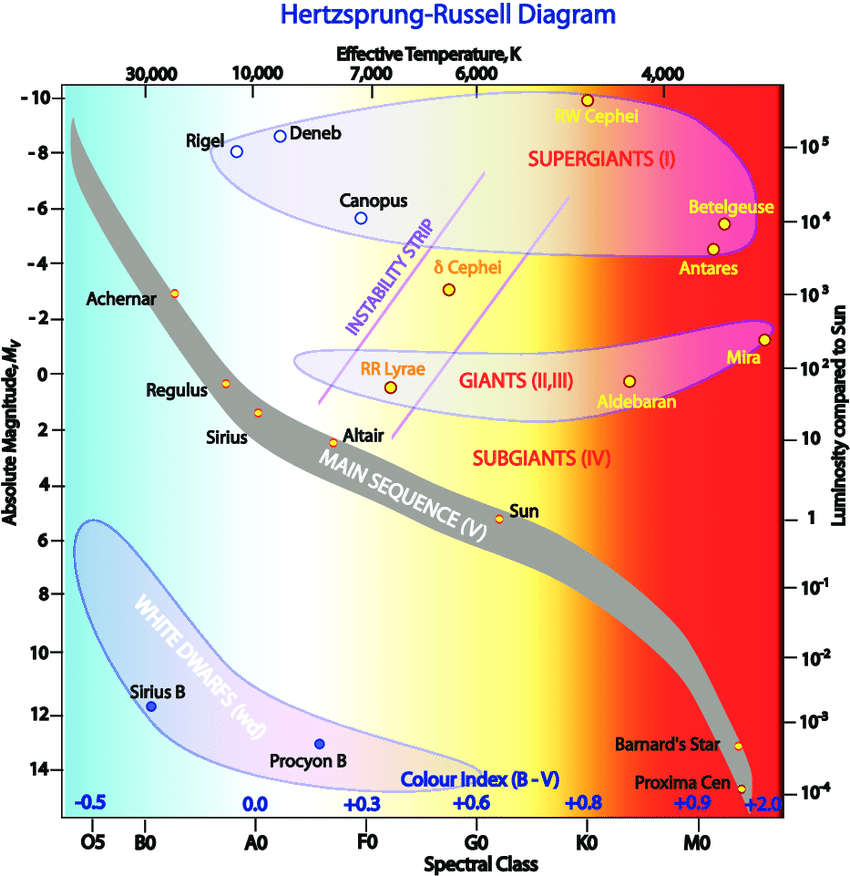
\includegraphics[width=\textwidth]{HRDAlthaus.png}
\caption[HR Diagram]{
\ac{HR} diagram as shown in figure 1 of \citet{Althaus2010}.
}
		\label{fig:Chap1:HRDAlthaus}
\end{figure}




\chapter{Paper I}
\label{chap:2}
\section{Introduction}
\label{sec:chap2:Introduction}
Section. Introduction of the topic of interest.

\subsection{Population Synthesis}
\label{subsec:chap2:popSynth}
Subsection.

\subsubsection{Rapid Population Synthesis}
\label{subsubsec:chap2:rapidPopSynth}
Subsubsection.

\begin{table}
\centering
\caption[Selection of observed properties of Galactic DNSs]{``Measured parameters of the Galactic \acp{DNS} used as a diagnosis in this study. ...
References: $^a$\citet{martinez2015pulsar}." Table extract as presented in \citealt{VignaGomez2018DNSs}} 
\label{tab:chap2:DNS}
\begin{tabular}{lcccccc}
\hline
Pulsar & $P$ & $e$ & $M_{\rm plsr}$  & $M_{\rm cmpn}$ & Ref \\
& $\rm [days]$ & & $\rm [M_{\odot}]$ & $\rm [M_{\odot}]$ &  \\
\hline
$\rm J0453+1559$ 			&	4.072	&	0.113	&	1.559	&	1.174	&	a	\\	
\end{tabular}
\end{table}

\chapter{Conclusions}
\label{chap:conclusions}
In this work we have unified physics.

\clearpage
\appendix
\label{chap:appendix}
\chapter{First Appendix}
Things that didn't make it to the main text.

\clearpage
\addcontentsline{toc}{chapter}{Bibliography}
\bibliography{thesis}
\bibliographystyle{abbrv}

\end{document}
